\documentclass{article}

\usepackage{booktabs}
\usepackage{inconsolata}
\usepackage{lineno}
\usepackage{todonotes}
\usepackage{xspace}
\usepackage{url}
\usepackage{alltt}
\usepackage{geometry}
\usepackage{enumitem}  
\usepackage{float}
\usepackage{color,soul}
\usepackage{listings}

\geometry{a4paper, margin=1in}


% Copyright 2017 Sergei Tikhomirov, MIT License
% https://github.com/s-tikhomirov/solidity-latex-highlighting/

\usepackage{listings, xcolor, inconsolata}

\definecolor{verylightgray}{rgb}{.97,.97,.97}

\lstdefinelanguage{Solidity}{
	keywords=[1]{anonymous, assembly, assert, balance, break, call, callcode, case, catch, class, constant, continue, contract, debugger, default, delegatecall, delete, do, else, emit, event, export, external, false, finally, for, function, gas, if, implements, import, in, indexed, instanceof, interface, internal, is, length, library, log0, log1, log2, log3, log4, memory, modifier, new, payable, pragma, private, protected, public, pure, push, require, return, returns, revert, selfdestruct, send, storage, struct, suicide, super, switch, then, this, throw, true, try, typeof, using, value, view, while, with, addmod, ecrecover, keccak256, mulmod, ripemd160, sha256, sha3}, % generic keywords including crypto operations
	keywordstyle=[1]\color{blue}\bfseries,
	keywords=[2]{address, bool, byte, bytes, bytes1, bytes2, bytes3, bytes4, bytes5, bytes6, bytes7, bytes8, bytes9, bytes10, bytes11, bytes12, bytes13, bytes14, bytes15, bytes16, bytes17, bytes18, bytes19, bytes20, bytes21, bytes22, bytes23, bytes24, bytes25, bytes26, bytes27, bytes28, bytes29, bytes30, bytes31, bytes32, enum, int, int8, int16, int24, int32, int40, int48, int56, int64, int72, int80, int88, int96, int104, int112, int120, int128, int136, int144, int152, int160, int168, int176, int184, int192, int200, int208, int216, int224, int232, int240, int248, int256, mapping, string, uint, uint8, uint16, uint24, uint32, uint40, uint48, uint56, uint64, uint72, uint80, uint88, uint96, uint104, uint112, uint120, uint128, uint136, uint144, uint152, uint160, uint168, uint176, uint184, uint192, uint200, uint208, uint216, uint224, uint232, uint240, uint248, uint256, var, void, ether, finney, szabo, wei, days, hours, minutes, seconds, weeks, years},	% types; money and time units
	keywordstyle=[2]\color{teal}\bfseries,
	keywords=[3]{block, blockhash, coinbase, difficulty, gaslimit, number, timestamp, msg, data, gas, sig, value, now, tx, gasprice, origin},	% environment variables
	keywordstyle=[3]\color{violet}\bfseries,
	identifierstyle=\color{black},
	sensitive=false,
	comment=[l]{//},
	morecomment=[s]{/*}{*/},
	commentstyle=\color{gray}\ttfamily,
	stringstyle=\color{red}\ttfamily,
	morestring=[b]',
	morestring=[b]"
}

\lstset{
	language=Solidity,
	backgroundcolor=\color{verylightgray},
	extendedchars=true,
	basicstyle=\ttfamily,
	showstringspaces=false,
	showspaces=false,
	numbers=left,
	numberstyle=\scriptsize\ttfamily,
	numbersep=9pt,
	tabsize=2,
	breaklines=true,
	showtabs=false,
	captionpos=b
}
% Copyright 2017 Sergei Tikhomirov, MIT License
% https://github.com/s-tikhomirov/solidity-latex-highlighting/

\usepackage{listings, xcolor, inconsolata}

\definecolor{verylightgray}{rgb}{.97,.97,.97}

\lstdefinelanguage{Solidity}{
	keywords=[1]{anonymous, assembly, assert, balance, break, call, callcode, case, catch, class, constant, continue, contract, debugger, default, delegatecall, delete, do, else, emit, event, export, external, false, finally, for, function, gas, if, implements, import, in, indexed, instanceof, interface, internal, is, length, library, log0, log1, log2, log3, log4, memory, modifier, new, payable, pragma, private, protected, public, pure, push, require, return, returns, revert, selfdestruct, send, storage, struct, suicide, super, switch, then, this, throw, true, try, typeof, using, value, view, while, with, addmod, ecrecover, keccak256, mulmod, ripemd160, sha256, sha3}, % generic keywords including crypto operations
	keywordstyle=[1]\color{blue}\bfseries,
	keywords=[2]{address, bool, byte, bytes, bytes1, bytes2, bytes3, bytes4, bytes5, bytes6, bytes7, bytes8, bytes9, bytes10, bytes11, bytes12, bytes13, bytes14, bytes15, bytes16, bytes17, bytes18, bytes19, bytes20, bytes21, bytes22, bytes23, bytes24, bytes25, bytes26, bytes27, bytes28, bytes29, bytes30, bytes31, bytes32, enum, int, int8, int16, int24, int32, int40, int48, int56, int64, int72, int80, int88, int96, int104, int112, int120, int128, int136, int144, int152, int160, int168, int176, int184, int192, int200, int208, int216, int224, int232, int240, int248, int256, mapping, string, uint, uint8, uint16, uint24, uint32, uint40, uint48, uint56, uint64, uint72, uint80, uint88, uint96, uint104, uint112, uint120, uint128, uint136, uint144, uint152, uint160, uint168, uint176, uint184, uint192, uint200, uint208, uint216, uint224, uint232, uint240, uint248, uint256, var, void, ether, finney, szabo, wei, days, hours, minutes, seconds, weeks, years},	% types; money and time units
	keywordstyle=[2]\color{teal}\bfseries,
	keywords=[3]{block, blockhash, coinbase, difficulty, gaslimit, number, timestamp, msg, data, gas, sig, value, now, tx, gasprice, origin},	% environment variables
	keywordstyle=[3]\color{violet}\bfseries,
	keywords=[4]{aspect, before, after, call-to, execution-of, add-to-declaration, update-definition, returning, in-interface, not-in-interface, get, set, tagged-with, originating-from, constructor},	% environment variables
	keywordstyle=[4]\color{orange}\bfseries,
	identifierstyle=\color{black},
	sensitive=false,
	comment=[l]{//},
	morecomment=[s]{/*}{*/},
	commentstyle=\color{gray}\ttfamily,
	stringstyle=\color{red}\ttfamily,
	morestring=[b]',
	morestring=[b]",	
	alsoletter=-
}

\lstset{
	language=Solidity,
	backgroundcolor=\color{verylightgray},
	extendedchars=true,
	basicstyle=\ttfamily,
	showstringspaces=false,
	showspaces=false,
	numbers=left,
	numberstyle=\ttfamily\scriptsize,
	numbersep=9pt,
	tabsize=2,
	breaklines=true,
	showtabs=false,
	captionpos=b
}
\lstset{
	basicstyle=\ttfamily%, columns=fullflexible
}

\newcommand{\AspectSol}{\textsc{AspectSol}\xspace}
\newcommand{\keyword}[1]{\textit{$\langle$#1$\rangle$}}
\newcommand{\tildearrow}{{\raise.37ex\hbox{$\scriptstyle\mathtt{\sim}$}}>\xspace}
\newcommand{\variable}[1]{\ensuremath{\langle\textrm{\textit{#1}}\rangle}}

\usepackage{todonotes}
\newcommand{\rf}[1]{\todo[color=red!25,size=\tiny]{#1 \textbf{/ Ryan}}}
\newcommand{\gp}[1]{\todo[color=green!25,size=\tiny]{#1 \textbf{/ Gordon}}}

\begin{document}
\title{\AspectSol v0.1$\alpha$\\User Manual}
\author{Gordon J. Pace and Joshua Ellul and Shaun Azzopardi and Ryan Falzon\\\texttt{\{gordon.pace|joshua.ellul|shaun.azzopardi\}@um.edu.mt, rfalzonryan@gmail.com}}
\date{published 1 August 2022, last updated 31 July 2022}
\maketitle

\tableofcontents

\section{Overview}	

Aspect oriented programming is a software development paradigm normally used in conjunction to object oriented programming. The main aim of such languages is to separate software concerns from the business layer to further increase code modularization. Typical cases where Aspect programming is beneficial is for logging and transactional logic. Such cases are not domain specific to the business logic and, when abstracted out, can in theory be used in any software you develop.

Given the nature of immutability of how blockchains operate, it makes developing smart contracts a tedious process as one would need to reach a level of confidence that the contract is bug free. Even though the majority of smart contracts are unique in terms of their behaviour, certain common factors might exist, such as for example admin-only calls to certain functions or even perhaps a number of steps that need to be taken following updates done to a balance. Hence, it would be beneficial if developers have access to a tool that allows them to program such non-business logic once, test it, and inject it into as many smart contracts as they want.

\AspectSol is an aspect-oriented language that aims at abstracting the implementation of features on top of already defined smart contracts to a higher level. This tool takes a script written in a domain language specified in this document and a Solidity smart contract, and produces a new Solidity smart contract reflecting the changes indicated in the aspect script. Such a tool allows for bulk updates of contracts where specific rules must be set on all of them.

The below is an example of the syntax used to formulate an \AspectSol script. In this example we see how one can inject code into a smart contract to make the \texttt{terminate} function executable only by the person who created the smart contract. Words such as \texttt{aspect}, \texttt{add-to-declaration}, \texttt{before} and \texttt{call-to} are all native keywords to the \AspectSol domain language. These, together with more, will be further described in section \ref{toolSyntax} of this manual.

\small\begin{lstlisting}[language=Solidity,numbers=left,numbersep=2pt,xleftmargin=0.3cm,label={code:aspectSolExample}, caption={\AspectSol Script Example.}]
	aspect OnlyOwnerInjection {
		address private owner;
		
		before execution-of Casino.constructor {
			owner = msg.sender;
		}
		
		before call-to Casino.terminate() {
			require(msg.sender == owner, "Caller is not owner");
		}
	}
\end{lstlisting}\normalsize
	
% \AspectSol is a tool which is still in an alpha stage where development on the tool is still ongoing. However, source code is being released as open source to encourage independent extensions and offshoots to the tool.

\section{Tool Syntax}
\label{toolSyntax}

The tool \AspectSol allows the for the creation of short function-like scopes called pointcuts. Within these scoped functions, one can include code that should be factored into the original smart contract based on whether the pointcut rule is met. Similar to how classes are created in OOP languages, in AOP languages, an Aspect needs to be created. Therefore a single aspect may contain several pointcuts. Code within pointcuts is then applied to smart contracts based on the rules set out in the pointcut definition.

\AspectSol provides two types of aspects: (i) \emph{code-appending} aspects which add advice (the new code) at the location of the pointcut, and (ii) \emph{modification} aspects which are used to update an existing definition of the original smart contract.

\subsection{Selector expressions}
\label{s:selectors}

In order to allow for the identification of pointcuts indicating where to append or modify the code, \AspectSol uses selector expressions to identify a relevant unit of code.
\[\begin{array}{lcl}
\variable{selector} & ::= &  \variable{contract-selector} \mid \variable{function-selector}
\end{array}\]

\paragraph{Contract selectors.}
Contract selectors are used to identify a subset of contracts in the source files \AspectSol is processing, with the following syntax (where the interface name is optional):
\[\begin{array}{lcl}
\variable{contract-selector} & ::= & \variable{contract-name}[::\variable{interface-name}]
\end{array}\]

A contract selector is made up of two components:
\begin{itemize}
    \item \textbf{Contract:} The contract selector specifies the name of the contract to match. It can be (i) a contract name to be matched in the source files provided; or (ii) a concrete address on the Ethereum blockchain where that contract is to reside. One can use \texttt{*} to match any contract name.
    \item \textbf{Interface:} The interface specifies that a smart contract will only match if it is an instance of the specified interface name. If no such restriction is desired, one can simply leave out the interface name (and preceding double colon symbol).
\end{itemize}

For instance, to identify the contract \texttt{CustomToken} which is to be an instance of \texttt{ERC20}, one would write \texttt{CustomToken::ERC20}. The contract selector \texttt{CustomToken} would match any contract so named in the source files, while \texttt{*::ERC20} would match all contracts which are instances of the \texttt{ERC20} interface.

\paragraph{Function selectors.}
Function selectors revolve around named contracts, defined contract interfaces and particular functions within contracts. A full function selector takes the following form (where the \texttt{returning} clause is optional):
\[\begin{array}{lcl}
\variable{function-selector} & ::= & \variable{contract-selector}.\variable{function-name}(\variable{parameters}) \;[\texttt{returning}\;\variable{type}]
\end{array}\]

For instance, to identify the \texttt{transfer} function in contract \texttt{CustomToken} which implements the \texttt{ERC20} interface, one would write:

\begin{alltt}
CustomToken::ERC20.transfer(address _to, address _amount) returning (bool)
\end{alltt}

The different components of the selector are discussed below:

\begin{itemize}
    \item \textbf{Function name:} This selector identifies which functions to match. If one wants to match \emph{all} functions in the specified contract, one can use the \texttt{*} symbol.
    \item \textbf{Parameters:} The parameters of the function can be identified, together with their type. The parameter names allow us access to the values passed in the advice. We can use the \texttt{*} symbol instead of a single parameter which we do not care about e.g. \texttt{CustomToken.transfer(address \_to, *)}, or to match the function with any number of parameters e.g. \texttt{CustomToken.transfer(*)}.
    \item \textbf{Return value:} The final part specifies the return type of the functions we want to match.\footnote{\textbf{Limitation:} We currently provide no means of accessing the return value in the advice, and only the type of the return value is specified.}  It can be left out altogether if one does not want to make any constraints. 
\end{itemize}

Below are some examples of function selectors: 

\begin{itemize}
    \item To match the parameterless \texttt{placeBet()} function in the \texttt{Casino} smart contract (which can be found in the sources provided to \AspectSol), one can use the selector \texttt{Casino.placeBet()}.
    \item To match all functions in the \texttt{Casino} smart contract, one can write: \texttt{Casino.*(*)}.
    \item If it is only parameterless functions in the \texttt{Casino} smart contract one is interested in, one would write: \texttt{Casino.*()}.
    \item In order to match any function called \texttt{withdraw} in any contract provided, one would use the selector: \texttt{*.withdraw(*)}.
    \item If one wants to identify functions of a smart contract already deployed ont he blockchain at a particular address, one would write: \texttt{0x71C7656EC7ab88b098defB751B7401B5f6d8976F.*(*)}.\footnote{Obviously, we cannot change the code of smart contracts already deployed, but we can use such selectors to identify, for instance, external calls to functions in such deployed contracts.} 
\end{itemize}

Sometimes, when one uses the wildcard selector \texttt{*}, one may want to access the actual name of that element. For instance, one may want to access the name of the function matching the selector \texttt{Casino.*()}. In order to do so, one can replace the wildcard with \texttt{[[f]]}, which binds the variable \texttt{f} with the name of the function in the rest of the pointcut (for instance to call the function again). Such bindings can be used with the contract and function names, including both in the same selector e.g. \texttt{[[cont]].[[func]](*)}.

In addition to selecting based on the contract and function names and parameters, \AspectSol also allows filtering selectors based on function decorators e.g. user modifiers, access modifiers, payable, etc. 

A selector can be followed by a decorator condition, written as: $\variable{selector}\;\texttt{tagged-with}\;\variable{decorator-expression}$.

Decorators allowed are: (i) access  modifiers (\texttt{public}, \texttt{private}, \texttt{internal}, \texttt{external}); (ii) function type modifiers (\texttt{pure} and \texttt{view}); (iii) the \texttt{payable} modifier; and (iv) user-defined modifiers. Decorator expressions are Boolean expressions over these base decorators, using 
 \texttt{\&} for conjunction, \texttt{|} for disjunction and \texttt{!} for negation. 
 
For instance, to select all public and external functions in the \texttt{Casino} smart contract which use the user-defined modifier \texttt{byOwner}, but which may not receive funds, one would write:
	
\begin{alltt}
Casino.*(*) tagged-with ((public | external) \& byOwner \& !payable)
\end{alltt}	

Finally, \AspectSol also provides means of filtering selectors to match only functions appearing (or not appearing) in a certain contract interface: writing $\variable{selector}\;\texttt{in-interface}\;\variable{interface-name}$ and $\variable{selector}\;\texttt{not-in-interface}\;\variable{interface-name}$.

For example, to select all public functions in the \texttt{CustomToken} smart contract which do not appear in the \texttt{ERC20} interface standard, one would write:
	
\begin{alltt}
CustomToken.*(*) not-in-interface ERC20 tagged-with public
\end{alltt}
	

% \[\begin{array}{lcl}
% \variable{function-selector} & ::= &
%     \variable{contract-identifier}.\variable{function-name}(\variable{parameters})\\
% \variable{contract-identifier} & ::= & 
%     \variable{contract-name} \mid \variable{contract-name} \texttt{::} \variable{interface-name}\\
% \variable{contract-name} & ::= &
%     \variable{bindable-wildcard} \mid 
%     \variable{identifier}\\
% \variable{interface-name} & ::= & 
%     \texttt{*} \mid \variable{identifier}\\
% \variable{function-name} & ::= & 
%     \variable{bindable-wildcard} \mid \variable{identifier}\\
% \variable{parameters} & ::= & 
%     \varepsilon \mid \texttt{*} \mid \variable{parameter-list}\\
% \variable{parameter-list} & ::= &
%     \variable{parameter} \mid 
%     \variable{parameter}\texttt{, }\variable{parameter-list}\\
% \variable{parameter} & ::= &
%     \variable{type}\;\variable{identifier}\\
% \variable{bindable-wildcard} & ::= &
%     \texttt{*} \mid \texttt{[[}\variable{identifier}\texttt{]]}
% \end{array}\]


\paragraph{Variable getter and setter selectors.}
Apart from functions, \AspectSol also allows selectors for global contract variable getters and setters. If such getters and setters are not defined in the code, \AspectSol creates them and replaces access to these variable using the new functions. Getter and setter selectors are identified using the following syntax:

\[\begin{array}{l}
\texttt{get}\;\variable{variable-type}\;\variable{contract-selector}.\variable{variable-name}\;[\texttt{tagged-with}\;\variable{decorator-expression}]\\
\texttt{set}\;\variable{variable-type}\;\variable{contract-selector}.\variable{variable-name}\;[\texttt{tagged-with}\;\variable{decorator-expression}]
\end{array}\]

Note that getter and setter selectors can be filtered using a decorator expression, but limited to the access modifiers \texttt{public}, \texttt{private} and \texttt{internal}.

As in the case of function selectors, the contract name, variable type and variable name can also be replaced by a wildcard or variable to capture the name. 

Below are some examples of selectors: 

\begin{itemize}
\item To capture all getters to the \texttt{savings} variable (of type \texttt{uint256}) in the \texttt{Wallet} smart contract, one would write: \texttt{get uint256 Wallet.savings}.
\item If one is interested in all setters to public variables named \texttt{savings} in any contract provided in the source, and of any type, one would write: \texttt{set * *.savings tagged-with public}.
\item To select all getters to \texttt{uint256} variables which are private or internal in any smart contract provided in the code, but also be able to refer the variable name, one would write:
\texttt{get uint256 *.[[var]] tagged-with (private | internal)}.
\end{itemize}

% When it comes to filtering out variable access, get and set selectors are available. As the name implies, the get selector matches any variable access within a smart contract and the set selector matches any variable modification in the smart contract. Due to the nature of how you would need to carry out the selection of gets and sets, the selectors differ slightly from what has been previously explained above:


\subsection{Identifying pointcuts}
\label{s:pointcuts}

Code-appending pointcuts identify locations in the code where advice can be injected. These pointcuts are encoded using selectors as follows:

\[\begin{array}{lcl}
\variable{pointcut} & ::= &
\variable{placement}\; \variable{location}\; \variable{function-selector}\; \variable{sender}
\end{array}\]

\noindent The components of such a pointcut are explained below:

\begin{itemize}
    \item \textbf{Placement:}
    The placement property dictates where the scoped code should be placed. Two options are available, \texttt{before} and \texttt{after}. The former triggers the advice code just \emph{before} the matched selection is executed, while the latter 
    triggers the advice code \emph{after} the matched selection. 
    
    \[\begin{array}{lcl}
        \variable{placement} & ::= & \texttt{before} \mid \texttt{after}
    \end{array}\]

    \item \textbf{Location:}
    The location property dictates whether the advice is inserted on the caller's side or as part of the selection, providing two options:  \texttt{call-to} and \texttt{execution-of}. This dictates the variables accessible from the advice.
    \begin{itemize}
	    \item \texttt{call-to} will inject the advice on the caller side of the matched selection (which has to be a function). The advice can thus access variables available on the caller's side. 
	    \item \texttt{execution-of}: As opposed to \texttt{call-to}, this will execute the advice at the start of the matched selection, thus having access to variable local to that selection.
    \end{itemize}

    \[\begin{array}{lcl}
        \variable{location} & ::= & \texttt{call-to} \mid \texttt{execution-of}
    \end{array}\]

    \item\textbf{Sender:} The sender property, written as \texttt{originating-from} $\variable{origin}$, is used to specify the originator of the smart contract call i.e. \texttt{msg.sender}. It is important to note that this property is optional. Different ways of identifying the origin of the call are available:
    
    \[\begin{array}{lcl}
        \variable{sender} 
        & ::=  & \texttt{originating-from}\; \variable{sender-source} \\
        \variable{sender-source} 
        & ::=  & \variable{address} \mid   \texttt{this} \mid \texttt{!this} \\
        & \mid & \variable{contract-selector} \mid \variable{function-selector} 
    \end{array}\]

    An Ethereum address can be used to specify the initiator of the transaction, expressed as a constant or using variables and functions available from the point where the joinpoint is instrumented e.g. the following pointcut refers to the start of calls to \texttt{depositMoney()} in the \texttt{Wallet} smart contract with \texttt{msg.sender} being the first entry in an array of owners, \texttt{owners[0]}:  

	\begin{alltt}
before execution-of Wallet.depositMoney() originating-from owners[0]
	\end{alltt}
	
	The expression (\texttt{owners[0]} in this case) is evaluated at the start of (\texttt{before}), and inside (\texttt{execution-of}) the \texttt{depositMoney()} function. 
	
	Checking whether or not the originating address is the same as the contract we are instrumenting can be checked using the \texttt{this} and \texttt{!this} sender identifier.
	
	The sender filter can also be used to restrict function call pointcuts to arise from within a particular function or contract, both specified by their name. For instance, the following two pointcuts match at the end of function \texttt{depositMoney()} of the contract named \texttt{Wallet} as long as the call originated from the \texttt{Bank} smart contract (which is to be defined in the source code provided to \AspectSol) or, more specifically, the \texttt{refund()} function in the \texttt{Bank} smart contract respectively:

    \begin{alltt}
after execution-of Wallet.depositMoney() originating-from Bank
after execution-of Wallet.depositMoney() originating-from Bank.refund()
    \end{alltt}
\end{itemize}

    While the above references function selectors, when it comes to variable access selectors, these can be only be used in conjunction with the placement property as follows:
    
    \begin{alltt}
after get uint256 Wallet.[[var\_name]]
    \end{alltt}



\subsection{Code injection aspects}
Using pointcuts, one can inject code at the locations by adding advice:

\[\begin{array}{lcl}
\variable{code-injection-aspect} & ::= &
\variable{pointcut}\; \texttt{\{} \variable{advice} \texttt{\}}
\end{array}\]

The code given in the advice is injected as is at matching pointcuts. For example, if one wants to keep count of how many times money is deposited in the \texttt{Wallet} smart contract using a \texttt{deposit} function and the running total of deposits one would write:
    \begin{alltt}
after execution-of Wallet.deposit(*) \{ 
    count\_deposits++;
    total\_deposits += msg.value;
\}
    \end{alltt}

It is worth noting that any variable with a binding in the pointcut can be  accessed in the advice using the same notation of the variable in double square brackets. All such occurrences in the advice are replaced by the term in the pointcut which matched. For instance, the following code emits an event whenever a \texttt{uint256} variable in the \texttt{Wallet} smart contract is updated:

    \begin{alltt}
after execution-of set uint256 Wallet.[[var\_name]] \{
  emit VariableRead("[[var\_name]]", [[var\_name]]);
\}
    \end{alltt}

\subsection{Code modification aspects}
Apart from adding executable code at a pointcut, \AspectSol also provides means of modifying existing code in a controlled manner. These aspects are defined over a logical block of code (typically defined as a selector), typically a function or a contract, which can be modified with appropriate advice.

\[\begin{array}{lcl}
\variable{modification-aspect} & ::= &
\texttt{add-to-declaration}\;\variable{selector}\;\{ \variable{declarations} \}\\
&\mid&
\texttt{update-definition}\;\variable{selector}\;\{ \variable{update-list} \}\\
\variable{update-list} & ::= & \varepsilon \mid \variable{update}\texttt{;}\;\variable{update-list}\\
\variable{update} & ::= & 
\texttt{implement}\;\variable{interface-name} \\
& \mid & \texttt{add-tag}\;\variable{decorator-name} \mid \texttt{remove-tag}\;\variable{decorator-name}
\end{array}\]

As can be seen above, \AspectSol provides two main modification types:

\begin{itemize}
	\item \texttt{add-to-declaration}: Add the advice code as part of the declaration of the matched selection. One can, for instance, declare new variables, modifiers, functions, etc. 
	\item \texttt{update-definition}: Allows updating the definition of the selected item using any combination of the following three directives:
	\begin{itemize}
		\item \texttt{add-tag} is used to add the named decorator (such as user defined modifiers and access control decorators) to the selected item.
		\item \texttt{remove-tag} is similarly used to remove the named decorator
		\item \texttt{implement} is used when one wants to make a given smart contract an instance of a given interface. This is typically accompanied with another \texttt{add-to-declaration} modification aspect which adds the definitions of the interface functions.  
	\end{itemize}
\end{itemize}

Some examples of modification aspects are the following:

\begin{itemize}
    \item In order to add a new variable to keep track of the number of times a function is called in a \texttt{Wallet} smart contract, one can use an \texttt{add-to-declaration} modification aspect:
    \begin{alltt}
add-to-declaration Wallet \{
    uint internal counter = 0;
\}
    \end{alltt}
    
    
    \item If one would want to make all private functions in the \texttt{Wallet} smart contract internal, one can add the following aspects:
    \begin{alltt}
update-definition Wallet.*(*) tagged-by private \{ 
   add-tag: internal; 
   remove-tag: private;
\}
    \end{alltt}
    
    \item In order to make the \texttt{CustomToken} an instance of the ERC20 token standard, one would write the following:
        \begin{alltt}
update-definition CustomToken \{
   implement: ERC20;
\}
    \end{alltt}

\end{itemize}

\subsection{Defining Aspects}
Aspects are defined as a sequence of pointcuts and advice meaning to achieve a common goal into one script. For instance, the following example shows how any changes to the variable keeping track of the owner and of whether the wallet is locked or not, can be guarded to ensure that they were initiated by the current wallet owner:

% \small\begin{lstlisting}[language=Solidity,numbers=left,numbersep=2pt,xleftmargin=0.3cm,label={code:aspectDefinitionSyntax}]
\begin{alltt}
aspect SafeWallet \{
   before set address Wallet.owner \{
     require(msg.sender == owner);
   \}

   before set bool Wallet.locked \{
      require(msg.sender == owner);
   \}
\}
\end{alltt}
	


\section{Tool Usage}

The process which is being followed involves the parsing of the input \AspectSol script file, followed by the parsing of the input Solidity smart contract file. This is followed by the \AspectSol execution and the new Smart Contract generation.

\begin{enumerate}
	\item \AspectSol Parsing: The first input to the tool should be a script file containing the code written in the \AspectSol scripting language. The script is firstly tokenized, after which the tokens are parsed to create an AST.
	\item Smart Contract Parsing: The second input to the tool is a Solidity smart contract. This contract is passed through solc compiler in order to also be parsed into an AST. However, the solc compiler also ensures that going forward we do not work on a smart contract which contains errors. Any errors generated by the solc compiler are displayed in the console for the user to inspect.
	\item \AspectSol Execution: In this stage, we take the \AspectSol AST and execute it based on the outputted smart contract AST. This is where the original smart contract is filtered and updated according to what was written in the \AspectSol script.
	\item Smart Contract Generation: Finally, once the smart contract AST has been updated accordingly, we again pass the smart contract AST back through solc to be able to re-generate a readable smart contract in Solidity.
\end{enumerate}

\subsection{Running \AspectSol}

After downloading the executable, the following is the procedure of running the tool:

\begin{enumerate}
    \item Identify path to \AspectSol script.
    \item Identify path to origin smart contract solidity file.
    \item Decide on the path to where the resulting smart contract solidity file should be written to.
    \item Open up a terminal window and navigate to the root folder of where the executable was downloaded to.
    \item Run the following command:
    
    \centerline{
        \texttt{aspectsol.exe \variable{path-to-aspect-script}} \variable{path-to-solidity-file} \variable{path-to-output-result}
    }
\end{enumerate}


\section{Use Cases}

In this section we present three use cases illustrating the use of \AspectSol.

\subsection{Use Case 1: Safe Variables}

One of the core principles of OOP is encapsulation. The general idea of this mechanism is that attributes of a class are kept private within the class. Read and write access to such attributes are made available from outside the class through functions. In OOP languages, such functions are more commonly referred to as getters and setters.

Consider the below solidity smart contract, where a custom token contract is created with a balance property. As it stands, the balance property is annotated with a public modifier, meaning anyone can read and update this property without any form of validation.

\small\begin{lstlisting}[language=Solidity,numbers=left,numbersep=2pt,xleftmargin=0.3cm,label={code:nonSafeVariableExample}, caption={Unsafe Variable Smart Contract.}]
	pragma solidity >=0.7.0 <0.9.0;
	
	contract CustomToken {
		
		public uint256 balance;
	}
\end{lstlisting}\normalsize
	
Let us consider that we want to change this so that reads and writes to the balance property need to go through a function first. Despite achieving the same thing, going through a function as opposed to directly accessing a property might be beneficial in cases were access needs to be given only to specific people, or when validation needs to be carried out prior to updating the value of a property.

\small\begin{lstlisting}[language=Solidity,numbers=left,numbersep=2pt,xleftmargin=0.3cm,label={code:safeVariableAspectSolScript}, caption={Safe Variable \AspectSol Script}]
  aspect SafeVariableInjection {					
      add-to-declaration CustomToken {
          function getBalance() public view returns(uint256) {
              return balance;
          }
      
          function setbalance(uint256 b) public {
              balance = b;
          }
      }
      
      update-definition CustomToken.balance tagged-with public {
          remove-tag: private
          add-tag: public
      }
  }
\end{lstlisting}\normalsize
	
Executing the above script would result in the original smart contract to be transformed to the below:

\small\begin{lstlisting}[language=Solidity,numbers=left,numbersep=2pt,xleftmargin=0.3cm,label={code:safeVariableContract}, caption={Safe Variable Smart Contract.}]
	pragma solidity >=0.7.0 <0.9.0;
	
	contract CustomToken {
		
		uint256 private balance;
		
		function getBalance() public view returns(uint256) {
			return balance;
		}
		
		function setbalance(uint256 b) public {
			balance = b;
		}
	}
\end{lstlisting}\normalsize

\subsection{Use Case 2: Ensuring Adherence to Business Process Flow}

Writing bug free smart contracts that adheres to their business process flow is of an utmost importance due to the nature of immutability that blockchains operate on. However, as important as it may be, this is very difficult to achieve. What we can do with \AspectSol, however is, provide a means of injecting reparations that can be performed in case of a violation to the business process flow.

Consider a Casino smart contract that allows for users to bet a certain amount of cryptocurrency tokens. An example of this contract can be seen below. In such a scenario, a logical or run-time bug might irreparable consequences. Therefore, it would be beneficial post-deployment that reparation actions are exposed.

\small\begin{lstlisting}[language=Solidity,numbers=left,numbersep=2pt,xleftmargin=0.3cm,label={code:casinoSmartContract}, caption={Casino Smart Contract.}]
	pragma solidity ^0.5.11;
	
	contract Casino{
		
		mapping(uint => mapping (uint => address payable[])) placedBets;
		mapping(uint => mapping(address => uint)) potShare;
		
		uint[] numbersGuessed;
		
		uint pot;
		
		uint tableID;
		uint tableOpenTime;
		
		address owner;
		
		constructor() public{
			owner = msg.sender;
		}
		
		function openTable() public{
			require(msg.sender == owner);
			require(tableOpenTime == 0);
			
			tableOpenTime = now;
			tableID++;
		}
		
		function closeTable() public{
			require(msg.sender == owner);
			require(pot == 0);
			
			delete numbersGuessed;
		}
		
		function timeoutBet() public{
			require(msg.sender == owner);
			require(now - tableOpenTime > 60 minutes);
			require(pot != 0);
			
			for (uint i = 0; i < numbersGuessed.length; i++) {
				uint l = placedBets[tableID][numbersGuessed[i]].length;
				
				for (uint j = 0; j < l; j++) {
					address payable better = placedBets[tableID][numbersGuessed[i]][l];
					better.transfer(potShare[tableID][better]);
					delete placedBets[tableID][numbersGuessed[i]];
				}
			}
			
			closeTable();
		}
		
		function placeBet(uint guessNo) payable public{
			require(msg.value > 1 ether);
			
			potShare[tableID][msg.sender] += msg.value;
			placedBets[tableID][guessNo].push(msg.sender);
			numbersGuessed.push(guessNo);
			pot += msg.value;
		}
		
		//we assume owner is trusted
		function resolveBet(uint _secretNumber) public{
			require(msg.sender == owner);
			
			uint l = placedBets[tableID][_secretNumber].length;
			if(l != 0){
				for (uint i = 0; i < l; i++) {
					placedBets[tableID][_secretNumber][i].transfer(pot/l);
				}
			}
			
			pot = 0;
			
			closeTable();
		}
	}
\end{lstlisting}\normalsize

Figure~\ref{f:business-process-casino} illustrates how the state of the contract changes depending on which function is called and by whom it was called. This is encoded in the format \texttt{party:function}. We can also see how states can only be transitiioned to if and only if the smart contract is in a particular state. For instance, calling the \texttt{withdrawFunds()} function is only allowed to be called by the \texttt{owner} when the smart contract is in a \texttt{NoBet} state. Using \AspectSol, we are able to encode this process flow in a script which would inject the necessary code to make this possible.

\begin{figure}[H]
    \centering
    \resizebox{!}{5cm}{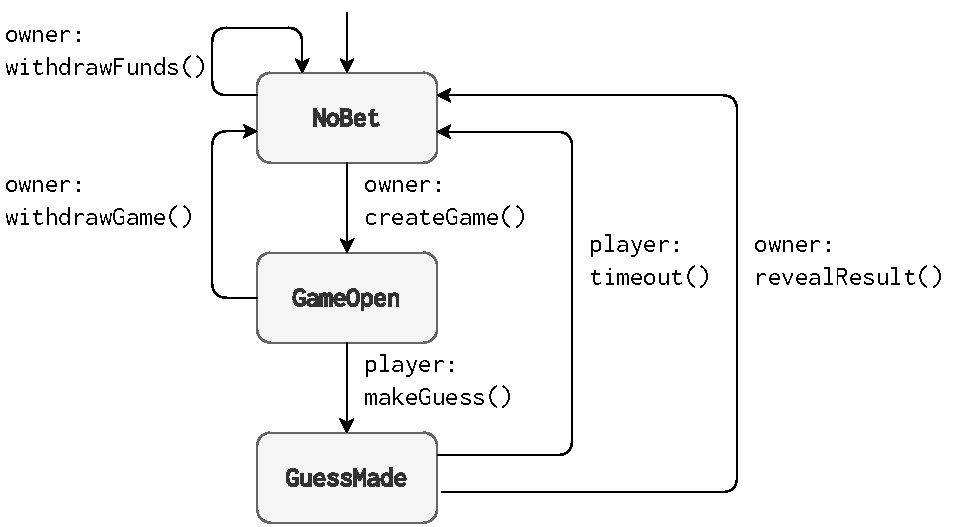
\includegraphics{images/casino-business-process-flow.pdf}}
    \caption{Casino business process}
    \label{f:business-process-casino}
\end{figure}

\small\begin{lstlisting}[language=Solidity,numbers=left,numbersep=2pt,xleftmargin=0.3cm,label={code:businessProcessFlowScript}, caption={Business Process Flow \AspectSol Script}]
    aspect OpenUntilResolution {
    	enum States {
    		TABLEOPEN,
    		TABLECLOSED,
    		BETPLACED,
    		TABLECLOSEDURINGBET
    	}
    
    	States currentState;
    
    	add-to-declaration Casino.openTable {
    		assert(currentState == States.TABLECLOSED);
    		currentState = States.TABLEOPEN;
    	}
    	
    	add-to-declaration Casino.closeTable {
    		assert(currentState == States.TABLEOPEN);
    		currentState = States.TABLECLOSED;
    	}
    	
    	add-to-declaration Casino.placeBet {
    		assert(currentState == States.TABLEOPEN);
    		currentState = States.BETPLACED;
    	}
    	
    	add-to-declaration Casino.resolveBet {
    		assert(currentState == States.BETPLACED);
    		currentState = States.TABLEOPEN;
    	}
    	
    	add-to-declaration Casino.timeoutBet {
    		assert(currentState == States.BETPLACED);
    		currentState = States.TABLEOPEN;
    	}
    }
\end{lstlisting}\normalsize
		
\subsection{Use Case 3: Reentrancy Free Contract}

Possibly one of the most fatal vulnerabilities for smart contracts is that of a reentrancy attack. Such a scenario would involve interaction between two contracts, a vulnerable one containing the reentrancy bug dubbed \textit{Contract A}, and a malicious one, which is ready to exploit the other's vulnerability referred to as \textit{Contract B}. \textit{Contract A} would send funds to \textit{Contract B}, which would trigger a fallback function in \textit{Contract B} that calls back into \textit{Contract A} before it is done updating balances.

A possible way of how you might go about mitigating this scenario, is by creating a boolean flag and use it to ensure that no code is executed while another transaction is currently being executed. Some choose to do this manually where and when needed, while others opt to create a modifier which does this manually every time a function is executed. Both approaches have their disadvantages: the former means that some instances may be unintentionally left out, whilst the latter is the equivalent of carpet bombing, disallowing calls between contract functions and unnecessarily increasing gas costs in functions which clearly do not yield control.

Using \AspectSol we show how this can be achieved for invocations to the \texttt{transfer} function:

\small\begin{lstlisting}[language=Solidity,numbers=left,numbersep=2pt,xleftmargin=0.3cm,label={code:reentracnyMitigationScript}, caption={Reentrancy Mitigation \AspectSol Script.}]
    aspect SafeReenentrancy {
        private bool running = false;
        
        before execution-of *.* { 
            require (!running);
        }
        
        before call-to *.transfer() {
            running = true;
        }
        
        after call-to *.transfer() {
            running = false;
        }
    }
\end{lstlisting}\normalsize
		
		
\section{\AspectSol Errors and Warnings}

The following are errors and warnings which \AspectSol may report:

\paragraph{10001} Failed to generate a valid token while compiling \AspectSol script. You may encounter this error if your \AspectSol script contains invalid syntax. Please refer to the line number provided with the error to help identify where the invalid syntax is located.

\paragraph{20001} Encountered a different token from what was expected while compiling the \AspectSol script. The error message template for this is \texttt{'Expected [\variable{expected-token}] but found: [\variable{actual-token}]'}. You may encounter this error if your \AspectSol script contains invalid syntax. Please refer to the line number provided with the error to help you identify where the invalid syntax is located.

\paragraph{30001} Placement token provided is not yet supported. Valid placement token values are \texttt{before} and \texttt{after}. Provided line number will indicate where the invalid placement token is located within the \AspectSol script.

\paragraph{30002} Location token provided is not yet supported. Valid location token values are \texttt{call-to} and \texttt{execution-of}. Provided line number will indicate where the invalid location token is located within the \AspectSol script.

\paragraph{30003} Variable access token provided is not yet supported. Valid variable access token values are \texttt{get} and \texttt{set}. Provided line number will indicate where the invalid variable access token is located within the \AspectSol script.

\paragraph{30004} Variable visibility token provided is not yet supported. Valid variable visibility token values are \texttt{public}, \texttt{private} and \texttt{internal}. Provided line number will indicate where the invalid variable visibility token is located within the \AspectSol script.

\paragraph{30005} Modification type token provided is not yet supported. Valid modification type token values are \texttt{add-to-declaration} and \texttt{update-definition}. Provided line number will indicate where the invalid modification type token is located within the \AspectSol script.
	
	
\section{Version History}

\begin{description}
	\item[0.1$\alpha$] released 1 August 2022 (First release)
\end{description}
	
\end{document}